\documentclass{beamer}

\usetheme{Rochester}
\usecolortheme{crane}

\usepackage{tikz}
\usepackage{ifthen}
\usepackage{tikz-3dplot}
\usepackage{pgfplots}

\usetikzlibrary{positioning}
\usepgfplotslibrary{dateplot}

\usepackage{siunitx}
\usepackage{wasysym}

\title{Timescales and Celestial Coordinates}
\author{Eivind Fonn}
\date{Juleseminar 2016}

\newcommand{\LST}{\text{LST}}
\newcommand{\GST}{\text{GST}}
\newcommand{\AXES}{
  \draw[tdplot_rotated_coords,red,->] (0,0,0) -- (2,0,0);
  \draw[tdplot_rotated_coords,green,->] (0,0,0) -- (0,2,0);
  \draw[tdplot_rotated_coords,blue,->] (0,0,0) -- (0,0,2);
}
\newcommand{\dd}{\text{d}}

\begin{document}

\frame{\titlepage}

\begin{frame}
  \frametitle{Goal}

  \begin{center}
    To convince you that the second, minute, hour, day and year are not units of
    time.
  \end{center}
\end{frame}

\begin{frame}
  \frametitle{Measuring time}

  To measure time we need a repeatable phenomenon with a consistent period.
  Typical choices are

  \begin{itemize}
  \item The motion of the sun with respect to an observer-local coordinate
    system on the Earth, one period of which is called a \emph{day}.
  \item The fluctuations of the seasons, one period of which is called a
    \emph{year}.
  \item The radiation corresponding to the transition between the two hyperfine
    levels of the ground state of caesium-133, $\SI{9192631770}{}$ periods of
    which are called an \emph{SI second}.
  \end{itemize}
\end{frame}

\begin{frame}
  \frametitle{Measuring time}

  \begin{itemize}
  \item A day is divided into 24 \emph{hours}, $\SI{1440}{}$ \emph{minutes} and
    $\SI{86400}{}$ \emph{seconds}.
  \item Likewise, 60 SI seconds is an \emph{SI minute}, $\SI{3600}{}$ SI seconds
    is an \emph{SI hour}, and $\SI{86400}{}$ SI seconds is an \emph{SI day}.
  \item The fact that a day can be split into a whole number of seconds, all of
    which are approximately equal to the SI second is ``pure coincidence.''
  \item The less said about the division of a year into a number of days, the
    better.
  \end{itemize}
\end{frame}

\begin{frame}
  \frametitle{Problems}

  \begin{itemize}
  \item The length of a year or a day are not only poorly defined, as we will
    see, they're also not consistent over time.
  \item As for caesium-133 radiation, it is comparatively difficult to observe
    by regular people, never mind counting to 9 billion in one second.
  \item Modern technology has solved the caesium-133 problem for us, but
    a way of controlling the motion of planets remains elusive.
  \end{itemize}
\end{frame}

\begin{frame}
  \frametitle{Coordinates}

  \begin{center}
    In a universe where everything that we can see moves, and everything is
    relative, how do we define any coordinates at all?
  \end{center}
\end{frame}

\begin{frame}
  \frametitle{Terminology}

  \begin{center}
    \tdplotsetmaincoords{70}{210}
    \begin{tikzpicture}[tdplot_main_coords]
      \begin{scope}
        \clip[tdplot_screen_coords] (0,0) circle (2);
        \shade[tdplot_screen_coords, ball color=gray, opacity=0.4] (-0.1,0) ellipse (2.4 and 2);
      \end{scope}

      \only<2->{
        \tdplotsetrotatedcoords{0}{23.4}{30}
        \draw[tdplot_rotated_coords,red] (2,0) arc (0:180:2);
        \draw[tdplot_rotated_coords,dotted,red] (-2,0) arc (180:360:2);
        \fill[tdplot_rotated_coords,red,opacity=0.1] (0,0) circle (2);
      }

      \only<3,5->{
        \tdplotsetrotatedcoords{0}{0}{30}
        \draw[tdplot_rotated_coords,blue] (2,0) arc (0:180:2);
        \draw[tdplot_rotated_coords,dotted,blue] (-2,0) arc (180:360:2);
        \fill[tdplot_rotated_coords,blue,opacity=0.1] (0,0) circle (2);
      }

      \only<4>{
        \tdplotsetrotatedcoords{10}{1.2}{20}
        \draw[tdplot_rotated_coords,blue,opacity=0.25] (2,0) arc (0:180:2);
        \draw[tdplot_rotated_coords,dotted,blue,opacity=0.25] (-2,0) arc (180:360:2);
        \fill[tdplot_rotated_coords,blue,opacity=0.025] (0,0) circle (2);
        \tdplotsetrotatedcoords{-10}{1.5}{40}
        \draw[tdplot_rotated_coords,blue,opacity=0.25] (2,0) arc (0:180:2);
        \draw[tdplot_rotated_coords,dotted,blue,opacity=0.25] (-2,0) arc (180:360:2);
        \fill[tdplot_rotated_coords,blue,opacity=0.025] (0,0) circle (2);
        \tdplotsetrotatedcoords{-2}{0.1}{32}
        \draw[tdplot_rotated_coords,blue,opacity=0.25] (2,0) arc (0:180:2);
        \draw[tdplot_rotated_coords,dotted,blue,opacity=0.25] (-2,0) arc (180:360:2);
        \fill[tdplot_rotated_coords,blue,opacity=0.025] (0,0) circle (2);
        \tdplotsetrotatedcoords{-20}{-0.7}{50}
        \draw[tdplot_rotated_coords,blue,opacity=0.25] (2,0) arc (0:180:2);
        \draw[tdplot_rotated_coords,dotted,blue,opacity=0.25] (-2,0) arc (180:360:2);
        \fill[tdplot_rotated_coords,blue,opacity=0.025] (0,0) circle (2);
      }

      \only<5>{
        \tdplotsetrotatedcoords{-90}{90}{90}
        \draw[tdplot_rotated_coords,black,fill=black,opacity=0.25]
        (0,0) -- (-2,0) arc (180:156.6:2) -- (0,0);
      }

      \only<6>{
        \draw[very thin] (0,-2) -- (0,2);
      }

      \only<7>{
        \draw[thick,yellow,->] (0,2) arc (90:138.59:2)
        node[midway,below] {$\alpha$};
        \tdplotsetrotatedcoords{48.59}{90}{90}
        \draw[tdplot_rotated_coords,thick,teal,->] (2,0) arc (0:70.58:2)
        node[midway,left] {$\delta$};
      }

      \only<8>{
        \draw[thick,yellow,->] (0,2) arc (90:138.59:2);
        \tdplotsetrotatedcoords{48.59}{90}{90}
        \draw[tdplot_rotated_coords,thick,teal,->] (2,0) arc (0:70.58:2);
        \tdplotsetrotatedcoords{0}{23.4}{70}
        \draw[tdplot_rotated_coords,thick,yellow,<-] (0,2) arc (90:20:2)
        node[midway,above left] {$\lambda$};
        \tdplotsetrotatedthetaplanecoords{90}
        \draw[tdplot_rotated_coords,thick,teal,->] (0,2) arc (90:40:2)
        node[midway,above right] {$\beta$};
      }

      \only<9-10>{
        \tdplotsetrotatedcoords{60}{-90}{0}
        \draw[tdplot_rotated_coords] (2,0) arc (0:158:2);
        \draw[tdplot_rotated_coords,dotted] (-2,0) arc (180:158:2);
      }

      \only<10>{
        \tdplotsetrotatedcoords{60}{0}{0}
        \draw[tdplot_rotated_coords,thick,yellow,->] (0,2) arc (90:50:2)
        node[midway,below] {$h$};
        \tdplotsetrotatedcoords{20}{90}{90}
        \draw[tdplot_rotated_coords,thick,teal,->] (2,0) arc (0:70:2)
        node[midway,left] {$\delta$};
      }

      \only<11>{
        \tdplotsetrotatedcoords{60}{-90}{0}
        \draw[tdplot_rotated_coords,black!50] (2,0) arc (0:158:2);
        \draw[tdplot_rotated_coords,dotted,black!50] (-2,0) arc (180:158:2);
        \tdplotsetrotatedcoords{80}{-90}{0}
        \draw[tdplot_rotated_coords] (2,0) arc (0:158:2);
        \draw[tdplot_rotated_coords,dotted] (-2,0) arc (180:158:2);
        \tdplotsetrotatedcoords{80}{0}{0}
        \draw[tdplot_rotated_coords,thick,yellow,->] (0,2) arc (90:30:2);
        \tdplotsetrotatedcoords{20}{90}{90}
        \draw[tdplot_rotated_coords,thick,teal,->] (2,0) arc (0:70:2);
      }

      \only<12>{
        \tdplotsetrotatedcoords{80}{-90}{0}
        \draw[tdplot_rotated_coords] (2,0) arc (0:158:2);
        \draw[tdplot_rotated_coords,dotted] (-2,0) arc (180:158:2);
        \tdplotsetrotatedcoords{80}{0}{0}
        \draw[tdplot_rotated_coords,thick,yellow,->] (0,2) arc (90:10:2)
        node[midway,below] {$\LST$};
      }

      \draw[tdplot_screen_coords,black,fill=blue!75,opacity=0.5] (0,0) circle[radius=0.07];
    \end{tikzpicture}
  \end{center}

  \only<1>{
    \begin{center}
      \emph{Celestial sphere}: the backdrop of far-away objects on the night
      sky. These move extremely slowly and can be considered fixed on a human
      development timescale.
    \end{center}
  }
  \only<2>{
    \begin{center}
      \emph{Ecliptic}: The trajectory traced out by the Sun on the celestial
      sphere over the course of a year. This is a great circle that moves
      somewhat over time.
    \end{center}
  }
  \only<3>{
    \begin{center}
      \emph{Equatorial plane}: The projection of Earth's equator onto the
      celestial sphere. This is also a great circle, and it moves quite
      significantly because the Earth doesn't ``rotate,'' it ``wobbles.''
    \end{center}
  }
  \only<4>{
    \begin{center}
      \emph{Precession} and \emph{nutation}: The ``long'' and ``short'' term
      movement of the equatorial plane, with principal periods of roughly
      $\SI{26000}{years}$ and $\SI{18.6}{years}$, respectively.
    \end{center}
  }
  \only<5>{
    \begin{center}
      \emph{Obliquity of the ecliptic}: The angle of intersection between the
      equatorial plane and the ecliptic, currently about $\SI{23.4}{\degree}$
      and increasing due to nutation.
    \end{center}
  }
  \only<6>{
    \begin{center}
      \emph{Equinoxes}: The points of intersection between the equatorial plane
      and the ecliptic. The one where the Sun moves to the northern hemisphere
      (the \emph{ascending node}) is the \emph{vernal equinox}.
    \end{center}
  }
  \only<7>{
    \begin{center}
      \emph{Equatorial coordinates}: Measured in terms of \emph{declination}
      $\delta$ (northern latitude) and \emph{right ascension} $\alpha$ (eastern
      longitude, from the equinox).
    \end{center}
  }
  \only<8>{
    \begin{center}
      \emph{Ecliptic coordinates}: Measured in terms of \emph{ecliptic
        longitude} $\lambda$ and \emph{ecliptic latitude} $\beta$. Not so useful
      for observers on Earth, for obvious reasons.
    \end{center}
  }
  \only<9>{
    \begin{center}
      \emph{Local meridian}: For a given observer, the plane that passes through
      the observer's zenith, and which is perpendicular to the equator. It
      rotates along with the earth.
    \end{center}
  }
  \only<10>{
    \begin{center}
      \emph{Local observer coordinates}: The same system as equatorial
      coordinates, only with the local meridian as the origin. The coordinate
      $h$ is referred to as the \emph{local hour angle}.
    \end{center}
  }
  \only<11>{
    \begin{center}
      Since the local meridian moves eastward along with the rotation of the
      Earth, the hour angle of anything increases by about one degree every four
      SI minutes.
    \end{center}
  }
  \only<12>{
    \begin{center}
      \emph{Local sidereal time (LST)}: The hour angle of the equinox. When
      measured on the Greenwich meridian, this is called \emph{Greenwich
        sidereal time} (GST).
    \end{center}
  }
\end{frame}

\begin{frame}
  \frametitle{For the mathies}

  As long as you know where you are, it's easy to convert:
  \[
    \LST = \GST + \lambda_\text{obs},
  \]
  where $\lambda_\text{obs}$ is the eastern longitude of the observer.
  Moreover,
  \begin{align*}
    h_\text{obj}
    &= \LST - \alpha_\text{obj} \\
    &= \GST + \lambda_\text{obs} - \alpha_\text{obj}.
  \end{align*}
  Note that, confusingly, the hour angle is measured \emph{westward}, unlike
  right ascension.
\end{frame}

\begin{frame}
  \frametitle{Solar time}

  \begin{center}
    \tdplotsetmaincoords{70}{210}
    \begin{tikzpicture}[tdplot_main_coords]
      \begin{scope}
        \clip[tdplot_screen_coords] (0,0) circle (2);
        \shade[tdplot_screen_coords, ball color=gray, opacity=0.4] (-0.1,0) ellipse (2.4 and 2);
      \end{scope}

      \tdplotsetrotatedcoords{0}{23.4}{30}
      \draw[tdplot_rotated_coords,red] (2,0) arc (0:180:2);
      \draw[tdplot_rotated_coords,dotted,red] (-2,0) arc (180:360:2);
      \fill[tdplot_rotated_coords,red,opacity=0.1] (0,0) circle (2);

      \tdplotsetrotatedcoords{0}{0}{30}
      \draw[tdplot_rotated_coords,blue] (2,0) arc (0:180:2);
      \draw[tdplot_rotated_coords,dotted,blue] (-2,0) arc (180:360:2);
      \fill[tdplot_rotated_coords,blue,opacity=0.1] (0,0) circle (2);

      \tdplotsetrotatedcoords{60}{-90}{0}
      \draw[tdplot_rotated_coords] (2,0) arc (0:158:2);
      \draw[tdplot_rotated_coords,dotted] (-2,0) arc (180:158:2);

      \only<1>{
        \tdplotsetrotatedcoords{60}{0}{0}
        \draw[tdplot_rotated_coords,yellow,thick,->] (0,2) arc (90:57.91:2)
        node[midway,below] {$h_{\text{sun}}$};
        \tdplotsetrotatedcoords{27.91}{90}{90}
        \draw[tdplot_rotated_coords,thick,teal,->] (2,0) arc (0:11.48:2);
        \tdplottransformmainscreen{-0.9174}{1.7320}{0.3981}
        \draw[tdplot_screen_coords,black,fill=yellow,opacity=0.75] (\tdplotresx,\tdplotresy) circle[radius=0.07];
      }

      \only<2>{
        \tdplotsetrotatedcoords{60}{0}{0}
        \draw[tdplot_rotated_coords,yellow,thick,->] (0,2) arc (90:72.53:2);
        \tdplotsetrotatedcoords{42.54}{90}{90}
        \draw[tdplot_rotated_coords,thick,teal,->] (2,0) arc (0:16.34:2);
        \tdplottransformmainscreen{-1.2973}{1.4143}{0.5627}
        \draw[tdplot_screen_coords,black,fill=yellow,opacity=0.75] (\tdplotresx,\tdplotresy) circle[radius=0.07];
      }

      \draw[tdplot_screen_coords,black,fill=blue!75,opacity=0.5] (0,0) circle[radius=0.07];
    \end{tikzpicture}
  \end{center}

  \only<1>{
    \begin{center}
      \emph{Local solar time}: The local hour angle of the sun. A constant
      offset of $\SI{12}{\hour}$ is often applied so that time ``zero'' is at
      midnight. Greenwich solar time is similarly defined.
    \end{center}
  }
  \only<2>{
    \begin{center}
      The Sun moves slowly eastward, which means that exactly one sidereal day
      later, the local solar time is slightly \emph{earlier}. In other words, a
      solar day is longer than a sidereal day.
    \end{center}
  }
\end{frame}

\begin{frame}
  \frametitle{Solar time}

  It is tempting to use Greenwich solar time as ``universal time.''
  Unfortunately, the angular speed
  \[
    \frac{\dd}{\dd t} h_{\text{sun}}(t)
  \]
  is not constant. Or, in other words, the right ascension of the sun is not
  increasing at a fixed rate. Why is this? There are two reasons.
\end{frame}

\begin{frame}
  \frametitle{The Equation of Time}

  \begin{itemize}
  \item The motion of the Sun across the ecliptic is due to the motion of the
    Earth around the Sun.
  \item Since Earth's orbit is elliptical, the orbital speed is slower at the
    apoapsis (early July) and faster at the periapsis (early January).
  \end{itemize}

  \begin{center}
    \begin{tikzpicture}
      \begin{axis}[
        width=\textwidth,height=0.5\textheight,
        axis lines=middle,
        ymin=-8,ymax=8,
        xtick={3.139,185.639},
        xticklabels={Periapsis,Apoapsis},
        ytick={-10,-5,0,5,10},
        minor y tick num={4},
        yticklabels={},
        grid=major,
        ]
        \addplot[blue,thick,mark=none] table[x index={1}, y index={2}]{eot.csv};
      \end{axis}
    \end{tikzpicture}
  \end{center}

  \begin{center}
    Length of solar day in seconds due to ellipticity.
  \end{center}
\end{frame}

\begin{frame}
  \frametitle{The Equation of Time}

  \begin{center}
    \tdplotsetmaincoords{70}{210}
    \begin{tikzpicture}[tdplot_main_coords]
      \begin{scope}
        \clip[tdplot_screen_coords] (0,0) circle (2);
        \shade[tdplot_screen_coords, ball color=gray, opacity=0.4] (-0.1,0) ellipse (2.4 and 2);
      \end{scope}

      \tdplotsetrotatedcoords{0}{23.4}{30}
      \draw[tdplot_rotated_coords,red] (2,0) arc (0:180:2);
      \draw[tdplot_rotated_coords,dotted,red] (-2,0) arc (180:360:2);
      \fill[tdplot_rotated_coords,red,opacity=0.1] (0,0) circle (2);

      \tdplotsetrotatedcoords{0}{0}{30}
      \draw[tdplot_rotated_coords,blue] (2,0) arc (0:180:2);
      \draw[tdplot_rotated_coords,dotted,blue] (-2,0) arc (180:360:2);
      \fill[tdplot_rotated_coords,blue,opacity=0.1] (0,0) circle (2);

      \tdplotsetrotatedcoords{0}{23.4}{0}
      \draw[tdplot_rotated_coords,yellow,thick,->] (0,2) -- (-0.5,2);
      \tdplottransformmainscreen{0}{2}{0}
      \draw[tdplot_screen_coords,black,fill=yellow,opacity=0.75] (\tdplotresx,\tdplotresy) circle[radius=0.07];

      \tdplotsetrotatedcoords{0}{23.4}{45}
      \draw[tdplot_rotated_coords,yellow,thick,->] (0,2) -- (-0.5,2);
      \tdplottransformmainscreen{-1.2973}{1.4143}{0.5627}
      \draw[tdplot_screen_coords,black,fill=yellow,opacity=0.75] (\tdplotresx,\tdplotresy) circle[radius=0.07];

      \tdplotsetrotatedcoords{0}{23.4}{90}
      \draw[tdplot_rotated_coords,yellow,thick,->] (0,2) -- (-0.5,2);
      \tdplottransformmainscreen{-1.8348}{0.0000}{0.7959}
      \draw[tdplot_screen_coords,black,fill=yellow,opacity=0.75] (\tdplotresx,\tdplotresy) circle[radius=0.07];

      \tdplotsetrotatedcoords{0}{23.4}{180}
      \draw[tdplot_rotated_coords,yellow,thick,->] (0,2) -- (-0.5,2);
      \tdplottransformmainscreen{-0.0000}{-2.0000}{0.0000}
      \draw[tdplot_screen_coords,black,fill=yellow,opacity=0.75] (\tdplotresx,\tdplotresy) circle[radius=0.07];

      \tdplotsetrotatedcoords{0}{23.4}{225}
      \draw[tdplot_rotated_coords,yellow,thick,->] (0,2) -- (-0.5,2);
      \tdplottransformmainscreen{1.2973}{-1.4143}{-0.5627}
      \draw[tdplot_screen_coords,black,fill=yellow,opacity=0.75] (\tdplotresx,\tdplotresy) circle[radius=0.07];

      \tdplotsetrotatedcoords{0}{23.4}{270}
      \draw[tdplot_rotated_coords,yellow,thick,->] (0,2) -- (-0.5,2);
      \tdplottransformmainscreen{1.8348}{-0.0000}{-0.7959}
      \draw[tdplot_screen_coords,black,fill=yellow,opacity=0.75] (\tdplotresx,\tdplotresy) circle[radius=0.07];

      \draw[tdplot_screen_coords,black,fill=blue!75,opacity=0.5] (0,0) circle[radius=0.07];
    \end{tikzpicture}
  \end{center}

  \only<1>{
    \begin{center}
      Even so, the speed of the Sun projected onto the equatorial plane will not
      be constant, but slower near the equinoxes and faster near the solstices.
    \end{center}
  }
\end{frame}

\begin{frame}
  \frametitle{The Equation of Time}

  This gives an even more pronounced effect.

  \begin{center}
    \begin{tikzpicture}
      \begin{axis}[
        width=\textwidth,height=0.5\textheight,
        axis lines=middle,
        ymin=-21,ymax=21,
        xtick={81.322,172.572,263.822,355.072},
        xticklabels={Equinox,Solstice,Equinox,Solstice},
        ytick={-20,-15,-10,-5,0,5,10,15,20},
        minor y tick num={4},
        yticklabels={},
        grid=major,
        ]
        \addplot[blue,thick,mark=none] table[x index={1}, y index={3}]{eot.csv};
      \end{axis}
    \end{tikzpicture}
  \end{center}

  \begin{center}
    Length of solar day in seconds due to the obliquity of the ecliptic.
  \end{center}
\end{frame}

\begin{frame}
  \frametitle{The Equation of Time}

  \begin{center}
    \begin{tikzpicture}
      \begin{axis}[
        width=\textwidth,height=0.7\textheight,
        axis lines=middle,
        ymin=-25,ymax=30,
        xtick={81.322,172.572,263.822,355.072},
        xticklabels={Equinox,Solstice,Equinox,Solstice},
        ytick={-25,-20,-15,-10,-5,0,5,10,15,20,25,30},
        minor y tick num={4},
        yticklabels={},
        grid=major,
        ]
        \addplot[blue,thick,mark=none] table[x index={1}, y index={4}]{eot.csv};
      \end{axis}
    \end{tikzpicture}
  \end{center}

  \begin{center}
    Length of solar day in seconds.
  \end{center}
\end{frame}

\begin{frame}
  \frametitle{The Equation of Time}

  \begin{center}
    \begin{tikzpicture}
      \begin{axis}[
        width=\textwidth,height=0.7\textheight,
        ymin=-18,ymax=18,axis lines=middle,
        xtick={81.322,172.572,263.822,355.072},
        xticklabels={Equinox,Solstice,Equinox,Solstice},
        ytick={-30,-25,-20,-15,-10,-5,0,5,10,15,20,25,30},
        minor y tick num={4},
        yticklabels={},
        grid=major,
        ]
        \addplot[blue,thick,mark=none] table[x index={1}, y index={5}]{eot.csv};
      \end{axis}
    \end{tikzpicture}
  \end{center}

  \begin{center}
    The difference in minutes between a \emph{mean} solar clock and an
    \emph{apparent} solar clock (a sundial) over the course of one year.
  \end{center}
\end{frame}

\begin{frame}
  \frametitle{The Mean Sun}

  \begin{itemize}
  \item The \emph{mean sun} is a theoretical point on the ecliptic whose right
    ascension increases at a constant rate.
  \item The long-term average of the difference between their right ascensions
    is zero.
    \[
      \left< \underbrace{\alpha_{\text{app.~sun}} - \alpha_{\text{mean sun}}}_{\text{EOT}} \right>_t = 0
    \]
  \end{itemize}
\end{frame}

\begin{frame}
  \frametitle{Mental gymnastics}

  \begin{align*}
    & \quad \text{Apparent solar days are longer} \\
    \Rightarrow & \quad \text{Apparent solar time increases more slowly} \\
    \Rightarrow & \quad \text{Mean solar time will appear to go faster} \\
    \Rightarrow & \quad \text{The mean Sun will appear to lag behind the apparent Sun} \\
    \Rightarrow & \quad \text{The apparent Sun is moving faster} \\
    \Rightarrow & \quad \text{Earth must rotate more to catch up with it every day} \\
    \Rightarrow & \quad \text{Apparent solar days are longer} \\
  \end{align*}
\end{frame}

\begin{frame}
  \frametitle{Universal time}

  Ok, so does \emph{mean} solar time increase at a constant rate?

  \begin{itemize}
  \item Close, but not really.
  \item Friction due to tidal forces slowly taps the Earth of rotational
    momentum, so mean (and apparent) solar days will keep getting longer as the
    Earth slows down.
  \item In addition to this there are seasonal variations due to atmospheric
    effects, and effectively random terms due to interactions between the crust,
    mantle and core.
  \end{itemize}
\end{frame}

\begin{frame}
  \frametitle{Universal time}

  \begin{itemize}
  \item UT1 (Universal time) is the time standard that measures mean solar time
    at the Greenwich meridian.
  \item In principle, there's no way to measure UT1 other than to do
    observations (because it's an \emph{angle}, not a \emph{time}).
  \item TAI (International Atomic Time) is the realization of the ideal time
    measured at mean sea level on Earth.
  \item In principle, there's no way to measure TAI other than to count
    caesium-133 radation periods (because it's a \emph{time}, not an
    \emph{angle}).
  \item However, TAI at least increases at a constant rate.
  \end{itemize}
\end{frame}

\begin{frame}
  \frametitle{Coordinated Universal Time}

  \begin{itemize}
  \item To create something that increases at a constant rate \emph{and} closely
    aligns with the mean solar time, we have Coordinated Universal Time (UTC).
  \item UTC is defined as a fixed offset from TAI, so it increases at the same
    rate TAI does.
  \item This offset is adjusted every now and then to keep UTC in close
    agreement with UT1. This is done by adding or removing a second on certain
    dates (last days of March, June, September and December).
  \item At the moment we need to add leap seconds once every few years. About
    $\SI{50000}{}$ years from now, we will need one leap second every day.
  \end{itemize}
\end{frame}

\begin{frame}
  \frametitle{$\text{UT1} - \text{UTC}$}

  \begin{center}
    \begin{tikzpicture}
      \begin{axis}[
        date coordinates in=x,
        width=\textwidth,height=0.7\textheight,
        axis y line=middle,
        axis x line=bottom,
        xticklabel={\year},
        grid=major,
        ]
        \addplot[blue, thick, mark=none]
        table[x index={22}, y index={8}]{data.csv};
      \end{axis}
    \end{tikzpicture}
  \end{center}

  \begin{center}
    The historical difference between UT1 and UTC.
  \end{center}
\end{frame}

\begin{frame}
  \frametitle{Length of Day (LOD)}

  \begin{center}
    \begin{tikzpicture}
      \begin{axis}[
        date coordinates in=x,
        width=\textwidth,height=0.7\textheight,
        axis y line=middle,
        axis x line=bottom,
        xticklabel={\year},
        grid=major,
        ]
        \addplot[blue, mark=none, very thin]
        table[x index={22}, y index={10}]{data.csv};
      \end{axis}
    \end{tikzpicture}
  \end{center}

  \begin{center}
    The excess length of a mean solar day (relative to an SI day) measured in
    milliseconds.
  \end{center}
\end{frame}

\begin{frame}
  \frametitle{A chart of the madness}

  \begin{center}
    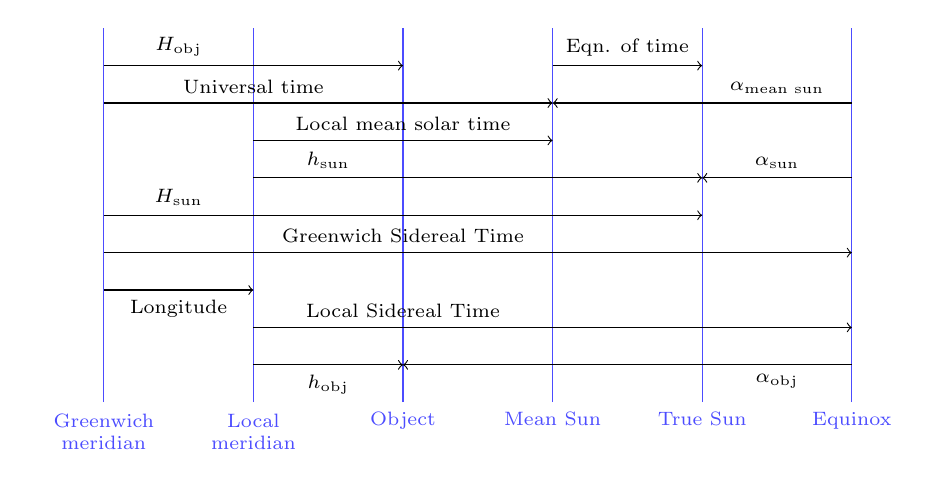
\begin{tikzpicture}[
      vlabel/.style={anchor=north,blue!70},
      hlabel/.style={anchor=south},
      vline/.style={thin,blue!70},
      scale=0.95,
      ]
      \def\gmer{0}
      \def\lmer{2}
      \def\x{4}
      \def\msun{6}
      \def\tsun{8}
      \def\eq{10}
      \draw[vline] (\gmer,0) -- (\gmer,5);
      \draw[vline] (\lmer,0) -- (\lmer,5);
      \draw[vline] (\x,0) -- (\x,5);
      \draw[vline] (\msun,0) -- (\msun,5);
      \draw[vline] (\tsun,0) -- (\tsun,5);
      \draw[vline] (\eq,0) -- (\eq,5);

      \node[vlabel] at (\gmer,0) {\scriptsize{\begin{tabular}{c}Greenwich\\meridian\end{tabular}}};
      \node[vlabel] at (\lmer,0) {\scriptsize{\begin{tabular}{c}Local\\meridian\end{tabular}}};
      \node[vlabel] at (\x,0) {\scriptsize{Object}};
      \node[vlabel] at (\msun,0) {\scriptsize{Mean Sun}};
      \node[vlabel] at (\tsun,0) {\scriptsize{True Sun}};
      \node[vlabel] at (\eq,0) {\scriptsize{Equinox}};

      \draw[->] (\gmer,4.5) -- (\x,4.5);
      \node[hlabel] at (\gmer+1,4.5) {\scriptsize{$H_\text{obj}$}};
      \draw[->] (\msun,4.5) -- (\tsun,4.5);
      \node[hlabel] at (\msun+1,4.5) {\scriptsize{Eqn. of time}};
      \draw[->] (\gmer,4.0) -- (\msun,4.0);
      \node[hlabel] at (\lmer,4.0) {\scriptsize{Universal time}};
      \draw[->] (\eq,4.0) -- (\msun,4.0);
      \node[hlabel] at (\tsun+1,4.0) {\scriptsize{$\alpha_\text{mean sun}$}};
      \draw[->] (\lmer,3.5) -- (\msun,3.5);
      \node[hlabel] at (\lmer+2,3.5) {\scriptsize{Local mean solar time}};
      \draw[->] (\lmer,3.0) -- (\tsun,3.0);
      \node[hlabel] at (\lmer+1,3.0) {\scriptsize{$h_\text{sun}$}};
      \draw[->] (\eq,3.0) -- (\tsun,3.0);
      \node[hlabel] at (\tsun+1,3.0) {\scriptsize{$\alpha_\text{sun}$}};
      \draw[->] (\gmer,2.5) -- (\tsun,2.5);
      \node[hlabel] at (\gmer+1,2.5) {\scriptsize{$H_\text{sun}$}};
      \draw[->] (\gmer,2.0) -- (\eq,2.0);
      \node[hlabel] at (\x,2.0) {\scriptsize{Greenwich Sidereal Time}};
      \draw[->] (\gmer,1.5) -- (\lmer,1.5);
      \node[hlabel,anchor=north] at (\gmer+1,1.5) {\scriptsize{Longitude}};
      \draw[->] (\lmer,1.0) -- (\eq,1.0);
      \node[hlabel] at (\x,1.0) {\scriptsize{Local Sidereal Time}};
      \draw[->] (\lmer,0.5) -- (\x,0.5);
      \node[hlabel,anchor=north] at (\lmer+1,0.5) {\scriptsize{$h_\text{obj}$}};
      \draw[->] (\eq,0.5) -- (\x,0.5);
      \node[hlabel,anchor=north] at (\tsun+1,0.5) {\scriptsize{$\alpha_\text{obj}$}};
    \end{tikzpicture}
  \end{center}
\end{frame}

\begin{frame}
  \frametitle{Fun fact: The zodiac}

  \begin{center}
    \tdplotsetmaincoords{55}{160}
    \begin{tikzpicture}[tdplot_main_coords]
      \begin{scope}
        \clip[tdplot_screen_coords] (0,0) circle (2);
        \shade[tdplot_screen_coords, ball color=gray, opacity=0.4] (-0.1,0) ellipse (2.4 and 2);
      \end{scope}

      \tdplotsetrotatedcoords{0}{0}{-20}
      \draw[tdplot_rotated_coords,blue] (2,0) arc (0:180:2);
      \draw[tdplot_rotated_coords,dotted,blue] (-2,0) arc (180:360:2);
      \fill[tdplot_rotated_coords,blue,opacity=0.1] (0,0) circle (2);

      \tdplotsetrotatedcoords{0}{23.4}{0}
      \draw[tdplot_rotated_coords,black,fill=black,opacity=0.5]
      (0,0) -- (0,2) arc (90:120:2)
      node[midway,below right,opacity=1,black] {\textbf{\aries}} -- (0,0);
      \tdplotsetrotatedcoords{0}{23.4}{30}
      \draw[tdplot_rotated_coords,black,fill=brown,opacity=0.5]
      (0,0) -- (0,2) arc (90:120:2)
      node[midway,right,opacity=1,black] {\textbf{\taurus}} -- (0,0);
      \tdplotsetrotatedcoords{0}{23.4}{60}
      \draw[tdplot_rotated_coords,black,fill=cyan,opacity=0.5]
      (0,0) -- (0,2) arc (90:120:2)
      node[midway,right,opacity=1,black] {\textbf{\gemini}} -- (0,0);
      \tdplotsetrotatedcoords{0}{23.4}{90}
      \draw[tdplot_rotated_coords,black,fill=green,opacity=0.5]
      (0,0) -- (0,2) arc (90:120:2)
      node[midway,above right,opacity=1,black] {\textbf{\cancer}} -- (0,0);
      \tdplotsetrotatedcoords{0}{23.4}{120}
      \draw[tdplot_rotated_coords,black,fill=magenta,opacity=0.5]
      (0,0) -- (0,2) arc (90:120:2)
      node[midway,above,opacity=1,black] {\textbf{\leo}} -- (0,0);
      \tdplotsetrotatedcoords{0}{23.4}{150}
      \draw[tdplot_rotated_coords,black,fill=olive,opacity=0.5]
      (0,0) -- (0,2) arc (90:120:2)
      node[midway,above,opacity=1,black] {\textbf{\virgo}} -- (0,0);
      \tdplotsetrotatedcoords{0}{23.4}{180}
      \draw[tdplot_rotated_coords,black,fill=orange,opacity=0.5]
      (0,0) -- (0,2) arc (90:120:2)
      node[midway,above left,opacity=1,black] {\textbf{\libra}} -- (0,0);
      \tdplotsetrotatedcoords{0}{23.4}{210}
      \draw[tdplot_rotated_coords,black,fill=pink,opacity=0.5]
      (0,0) -- (0,2) arc (90:120:2)
      node[midway,left,opacity=1,black] {\textbf{\scorpio}} -- (0,0);
      \tdplotsetrotatedcoords{0}{23.4}{240}
      \draw[tdplot_rotated_coords,black,fill=teal,opacity=0.5]
      (0,0) -- (0,2) arc (90:120:2)
      node[midway,left,opacity=1,black] {\textbf{\sagittarius}} -- (0,0);
      \tdplotsetrotatedcoords{0}{23.4}{270}
      \draw[tdplot_rotated_coords,black,fill=violet,opacity=0.5]
      (0,0) -- (0,2) arc (90:120:2)
      node[midway,below left,opacity=1,black] {\textbf{\capricornus}} -- (0,0);
      \tdplotsetrotatedcoords{0}{23.4}{300}
      \draw[tdplot_rotated_coords,black,fill=red,opacity=0.5]
      (0,0) -- (0,2) arc (90:120:2)
      node[midway,below,opacity=1,black] {\textbf{\aquarius}} -- (0,0);
      \tdplotsetrotatedcoords{0}{23.4}{330}
      \draw[tdplot_rotated_coords,black,fill=white,opacity=0.5]
      (0,0) -- (0,2) arc (90:120:2)
      node[midway,below,opacity=1,black] {\textbf{\pisces}} -- (0,0);

      \draw[tdplot_screen_coords,black,fill=blue!75,opacity=0.5] (0,0) circle[radius=0.07];
    \end{tikzpicture}
  \end{center}

  \only<1>{
    \begin{center}
      The zodiac sign you are born into is determined by the $\SI{30}{\degree}$
      sector the Sun is in when you're born. They are named after constellations
      that are found roughly in those directions.
    \end{center}
  }
  \only<2>{
    \begin{center}
      The equinox is also known as the \emph{first point of Aries} (\aries),
      because that's literally what it is. Except the equinox has moved so much
      by now that it's not in the constellation Aries any more.
    \end{center}
  }
  \only<3>{
    \begin{center}
      Most astrologists seem to have decided that it's more important that the
      sectors move with the equinox (the tropical zodiac) than with the actual
      constellations (the sidereal zodiac).
    \end{center}
  }
\end{frame}

\end{document}
